\documentclass[12pt,fleqn]{article}
\usepackage{graphicx}
\setlength{\parindent}{0pt}
\setlength{\parskip}{8pt}
\setlength{\parsep}{0pt}
\setlength{\headsep}{0pt}
\setlength{\topskip}{0pt}
\setlength{\topmargin}{0pt}
\setlength{\topsep}{0pt}
\setlength{\partopsep}{0pt}
\setlength{\mathindent}{0cm}
\usepackage{listings}

\begin{document}

Ders 1

Birinci derece normal diferansiyel denklemler (ordinary differential equtions
-ODE-) standart formunda $y'=f(x,y)$ gibi dururlar (bu form her zaman
elde edilemeyebilir, ama simdilik yapilabildigini kabul edelim).  Mesela

\[ y' = \frac{x}{y'} \] 

ya da

$y' = x-y^2$ 

ya da

$y' = y-x^2$

Bu denklemlerden birincisi degiskenleri ayirma (seperation of variables)
yontemiyle rahatca cozulebilir. 2. ve 3. denklemlerde bu yapilamaz. 3. denklem
baska bir sekilde kolayca cozulebilir, ama 2. analitik, formulsel olarak
cozulemez. Yani daha ise baslar baslamaz en basit gozuken, sadece birinci derece
turevi iceren ODE'de bile analitik cozum olamayacagini goruyoruz. Bu formulu
ileride numerik olarak cozecegiz.

Ve bu tur formuller matematikte istisna olmaktan ziyade kural sayiliyorlar (yani
cok karsimiza cikiyorlar). 

Simdi ODE'lere geometrik ve numerik olarak bakmanin yollarini gorecegiz.

Diyelim ki elimizde $y' = f(x,y)$ ODE'si var. Cozumlerden birinin
$y_1(x)$ oldugunu dusunelim. Geometrik olarak 

\begin{tabular}{cc}
Analitik & Geometrik \\ \hline
$y' = f(x,y)$ & Yon Alanlari (Direction Field) \\
$y_1(x)$. & Entegral Egrileri (Integral Curves)
\end{tabular}

Entegral egimleri nasil cizilir? Her $x,y$ icin $f(x,y)$'in verdigi deger o
noktaya tekabul eden yerde bir ``egim (slope)'' olarak kabul edilir, ve o egime
gore o noktada cizilir. Rasgele bir resim altta.

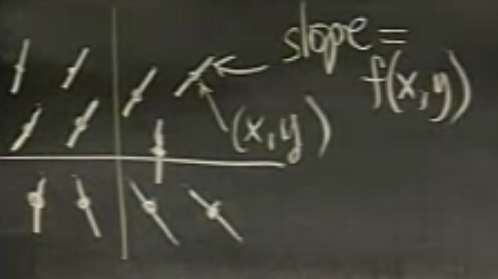
\includegraphics[height=4cm]{./1_1.png}

Sonra bu egim parcaciklarina ``her noktada'' teget gecen cizgiler cizilir
(kirmizi renkliler), bunlar entegral egimleridir.

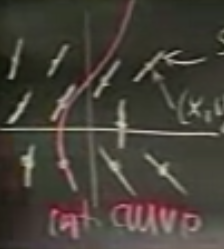
\includegraphics[height=4cm]{./1_2.png}

Bir entegral egimi, bir analitik cozume esdegerdir. Teorisel olarak $y_1(x)$
$y'=f(x,y)$ icin bir cozumdur, sadece ve sadece $y_1(x)$'in grafigi bir entegral
egri ise. Ispat: $y_1(x)$'i ODE icine koyalim, $y_1(x) = f(x,y_1(x))$. Peki
$y_1(x)$'in egimleri nelerdir? Bu egim $f(x,y_1(x))$'tir. Iki taraf birbirine
esit olduguna gore entegral egrileri ve analitik cozum birbirine esittir.

Bu egimleri nasil cizeriz? Bilgisayar soyle yapar: bir x,y secer, o x,y icin
f(x,y)'yi mekanik olarak hesaplar ve o noktada bir egim cizer. Insan ne yapar:
Bir ``egim'' $c$ onceden ``secer'', ve o $f(x,y)=c$ icin bu formule uyacak
$f(x,y)$ ve onun uzerindeki egim parcalarini birlestirerel cizmeye ugrasir.

Ornek: 

\[ y' = \frac{-x}{y} \]

\[ \frac{-x}{y} = c \]

\[ y = \frac{-1}{c}x \]

c=1 icin 0,0 noktasindan gecen bir cizgi vardir.

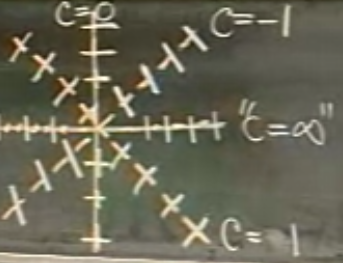
\includegraphics[height=4cm]{./1_3.png}

O zaman entegral egrileri neye benzer? Bir cembere. Hatta degisken ayirma
(seperation of variables) yontemiyle cozseydik, sonuc $x^2+y^2=c^2$ turunde
olacakti ki bu bir cemberin formuludur.

Bir baskasi

$y' = 1+x-y$

Bir c icin egimler

$y = 1+x-c$ ya da

$y = x+(1-c)$

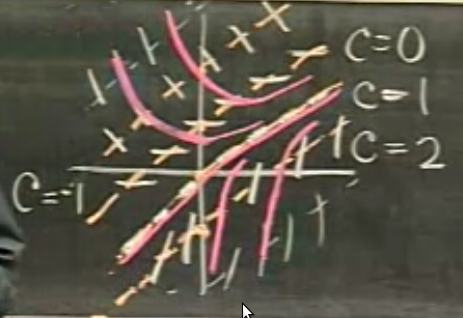
\includegraphics[height=4cm]{./1_4.png}

Entegral egrilerini cizerken bazi kurallar vardir: Biri, entegral egrileri
cakisamazlar. Niye? Bu olabilseydi bir x,y noktasinda iki ayri egim
hesaplanabilir demek olacakti, fakat elimizde tek bir $f(x,y)$ fonksiyonu
var. Demek ki bu mumkun degil.

Ayrica asimptotik olarak (sonsuza giderken) x sonsuza giderken egrilerin sag
tarafta bir yone dogru gruplandigini, meyil ettigini goruyoruz. $y=x$'e dogru
toparlaniyorlar. Demek ki $y=x$ bir cozumdur. Kontrol edelim, diferansiyel
denkleme koyarsak,

$y' = 1+x-y$

$x' = 1+x-x$

$1 = 1$

Demek ki $y=x$ bir cozum ve bunu sadece geometriye bakarak anladik. 

Ikinci kural: iki entegral egrisi birbirlerine tanjant bile olamazlar, yani
birbirlerine dokunamazlar. Ispat mevcudiyet ve ozgunluk kanunu (existence and
uniquiness theorem). Teori der ki $x_o, y_o$ noktasinda $y'=f(x,y)$'in bir ve
sadece bir tane cozumu vardir. 

Ornek: 

$xy' = y - 1 $

\[ \frac{dy}{y-1} = \frac{dx}{x} \]

Iki tarafin entegralini al

$ln|y-1| = ln|x| + c_1$

$y=1 = cx$

$y = 1-cx$


Cozum neye benzer? y=1 noktasindan gecen her turlu duz cizgi bir cozumdur. 

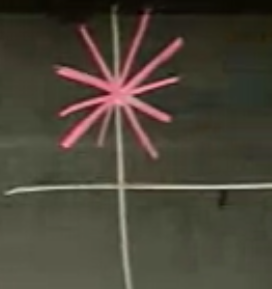
\includegraphics[height=4cm]{1_5.png}

Fakat y kordinati tamami uzerinde cozum yoktur. Kesisme olan noktada ise
ozgunluk yoktur. Yanliz diferansiyel denklemi $\frac{dy}{dy}$ solda olacak
sekilde, formda tanimlamamiz lazim. 

\[ \frac{dy}{dy} = \frac{y-1}{x} \]

O zaman bu formulde x=0 noktasinda formulun surekliliginin olmadigini (not
continuous) goruyoruz, ve hakikaten de bu sureksizlik diferansiyel denklemin
cozumunde mevcudiyet ve ozgunlugun bozuldugu yer ile ayni. 

ODE dunyasinda bu cozumsuz noktalar her zaman ortaya cikabiliyorlar. 

Grafik

Altta $y' = y^2-x$ formulunun vektor akis diyagramini grafiklemek icin
kullanilan Python kodlarini bulabilirsiniz.

\lstinputlisting[language=Python]{isoclines.py}

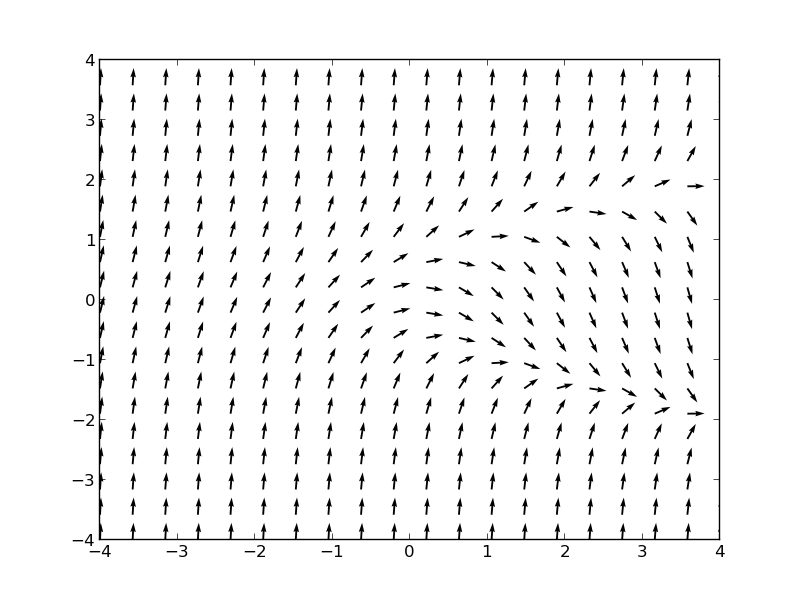
\includegraphics[height=8cm]{isoclines.png}

\end{document}


